\section{Controllability}
Control systems face numerous challenges, including stabilizing unstable systems through feedback control. Controllability is a crucial factor in addressing these challenges. A system is considered controllable if a single control input, denoted as 'u', can effectively steer the system's state from any initial configuration to any desired final state. For a linear time-invariant state-space system to be controllable, the controllability matrix 'P' must have full rank, which implies that its rank must equal the number of states ('n') in the system.\newline

$\mathcal{C} = \left[ \begin{matrix}
	B & AB & A^2B & \cdots & A^{n-1}B
\end{matrix} \right]$

$rank(\mathcal{C}) = n$


\begin{verbatim}
	% MATLAB script
	ms  = 34;           % Sprung Mass (kg)
	mus = 11;           % Unsprung Mass (kg)
	ks  = 6921;         % Suspension Stiffness (N/m)
	kus = 81000;        % Wheel stiffness (N/m)
	bs  = 0;            % Suspension Inherent Damping coefficient (sec/m)
	bus = 0;            % Wheel Inhenrent Damping coefficient (sec/m)
	
	%% System Dynamics for the Active Suspension system.
	A = [ 0 1 0 -1 ;
		-ks/ms -bs/ms 0 bs/ms;
		0 0 0 1; 
		ks/mus bs/mus -kus/mus -(bs+bus)/mus];
	
	B = [0  0 ; 
		0 1/ms ; 
		-1  0 ;
		bus/mus -1/mus ];
		
	C = [ 1 0 0 0 ; 
		-ks/ms -bs/ms 0 bs/ms ];
	
	D = [0 0;
		0 0;
		0 0;
		0 0;
		0 0;
		0 1/ms];
	
	%% Controllability
	rank(ctrb(A,B))
\end{verbatim}

\newpage
The following figure shows that the system is controllable, because its controllability matrix is full rank which is equal to the number of states.

\begin{figure}[H]
	\centering
	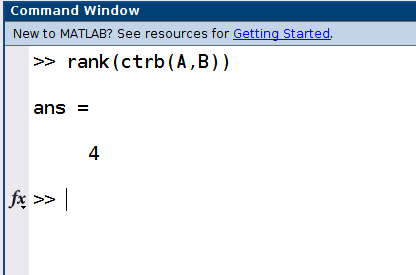
\includegraphics[width=0.4\textwidth]{ctrb.png}
	\caption{Conrollability matrix is full rank}
	\label{fig:ctrb}	
\end{figure}


\section{Full State Feedback}
A full state feedback controller, also referred to as a pole placement controller which is shown in figure \ref{fig:stfb}, provides an optimal solution for achieving desired pole locations of a closed-loop system. This approach leverages the fact that all state variables are assumed to be known to the controller at all times and are available for feedback.

The state-space representation of the plant is utilized, where each state variable is fed back to the control input, u, through a gain matrix, K. This feedback gain matrix can be adjusted to achieve the desired closed-loop pole values.

\begin{figure}[H]
	\centering
	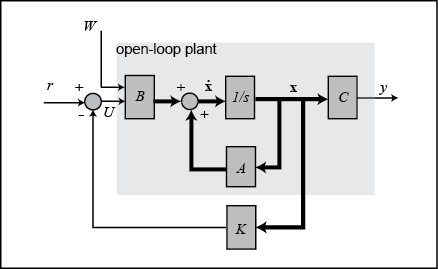
\includegraphics[width=0.4\textwidth]{stfb.png}
	\caption{Full state feedback block diagram. \cite{controltutorials}
	}
	\label{fig:stfb}
\end{figure}

Assuming no tracking $(r=0)$ and no external disturbance $(w=0)$, the system input is given by:

$u = -Kx$

$\dot{x} = Ax - BKx$

$\dot{x} = x(A - BK)$

\section{Linear Quadratic regulator (LQR)}
A widely used type of state feedback control that offers a systematic method for determining the control gain, $K$, is LQR controller. The LQR approach will be employed in the controller design for the active suspension system, as it is a classic and straightforward option for linear, time-invariant, multiple-input multiple-output (MIMO) systems. One of the key advantages of using an LQR controller is its ability to weight the factors affecting the performance index based on the desired outcome. For this project, the focus of the LQR approach will be on enhancing ride comfort and improving road-handling performance in the quarter-car model.

\newpage
The function of an LQR controller is to minimize the cost function, J, which is shown in the following equation:

\[
J = \frac{1}{2} \int_{0}^{t} (x^{T}Qx + u^{T}Ru) \, dt 
\]

$x^{T}$ = State vector. 

$u^{T}$ = Input vector.


\subsection{LQR Implementation}
The weighting matrices, Q and R, within the quadratic performance index significantly influence the LQR controller's behavior. These matrices allow for tuning the control system's priorities, such as emphasizing ride comfort or minimizing control effort. The optimal values for Q and R were determined through iterative simulations and tuning within the MATLAB environment. This process involved systematically adjusting the elements of Q and R and observing the resulting system response to determine the combination that best met the desired performance objectives.


